\chapter{Validation in liquid jet in crossflow}
	\label{ch6:jicf_lgs_simulations}


Describe here all our results from the lagrangian simulations:

\begin{itemize}

	\item Effects of applying full workflow: w/wo ALM, w/wo secondary atomization ...
	
	\item Mesh convergence study: specify it
	
	\item Validation with experiments
	
	\item Mass conservation issues: lagrangian tracking, etc. 
	

\end{itemize}



\section{Introduction}

The mesh shown in Figure \ref{fig:jicf_dlr_mesh} is used. However, this grid shows a baseline cell size downstream liquid injection coarser to the upstream region, which will affect the resolution of the gaseous field. Another mesh should be used for this study, this is discussed in the mesh convergence section.

The operating points simulated are those from Figure \ref{tab:jicf_operating_conditions}.

\subsection{Evaporation phenomena}

\textbf{Note: this analysis could perfectly be in the previous chapter}.

As indicated in Table \ref{tab:jicf_operating_conditions}, the temperatures of both liquid kerosene and gaseous air are low (290 and 288 K respectively) and there is not direct evaporation of fuel. Nevertheless, some evaporation can occur at ambient temperature if the vapour pressure of the liquid is lower than the ambient pressure. In the experiments, the ambient pressure is $p_g = 6$ bar, while the vapour pressure of kerosene at $288$ K is $p_{vap} = 0.003$ bar \citepColor[shepherd_flash_2000]. Therefore, evaporation might be possible.

It is tested that ... Two characteristic times are used in the low We case (since the lowest velocity is found there, and the droplets take more time to reach the validation plane at 80 mm)/

\begin{itemize}

	\item The time that a droplet takes to reach the plane x = 80 mm. From the SPS results in $\S$\textbf{??} (or Table \textbf{??}), the first droplets at x = 10 mm are obtained at $t_{resolv} = 0.3$ ms after injection. Then, the first droplets injected at this location in the lagrangian simulations reach the validation plane after $t_\mathrm{lagr} = $ ms. Hence, a characteristic time defined as the :
	
	\begin{equation}
	\tau_{validation} = t_{resolv}  + t_\mathrm{lagr}
	\end{equation}
	
	\item Evaporation time rate is used by means of the $d^2$ law. This law that the square of the droplet's diameter diminishes linearly with time:
	
	\begin{equation}
	\label{eq:d2_law}
	d^2 \left( \right) = d_0^2 - K t
	\end{equation}
	
	
	where $K$ is the evaporation rate and $d_0$ the initial diameter of the droplet. The value K ... (see 2006 Ghassemi).
	
	
	\text{NAH}. The evolution in diameter after a given time $t$ can then be obtained as:
	
	\begin{equation}
	\Delta d^2 = d_0^2 - d^2 \left( \right) = K t
	\end{equation}
	

\end{itemize}

\section{Blockage effect modeling}

\section{Relation between volume and mixture fractions}

So we can relate $\overline{\alpha}$ field with the mixture fraction somehow, this will be interesting for people doing combustion. I have developed the following relation between mixture fraction $Z$ and volume fraction $\alpha$ (need to check it properly):

\begin{equation}
Z = \frac{m_F}{m_F + m_A} = \frac{V_F \rho_F}{V_F \rho_F + V_A \rho_A} = \frac{1}{1 + \frac{V_A}{V_F} \frac{\rho_A}{\rho_F}} = \frac{1}{1 = \frac{\rho_A}{\rho_F} \frac{1 - \alpha}{\alpha}}
\end{equation}


We can also make a link to heat relase, for the interest of combustion studies.


\section{Models sensitivity}

ALSO: effect of one and two-way coupling !! Ver articulos 2010, 2011 Li 

\subsection{Effect of injection conditions}

\subsection{Effect of secondary atomization model}

\subsection{Effect of dense core blockage effect model}

\section{Results}

\subsection{Mesh convergence study}

\subsection{Validation with experiments (quantitative/qualitative)}

\subsection{Trajectories}

In order to illustrate the lagrangian trajectories and the continuity with respect to the resolved jets, a volume fraction field can be defined in the lagrangian simulations:

\begin{equation}
\alpha_l \left( \textbf{x}, t \right) = \frac{V_l \left( \textbf{x}, t \right)}{V_{el}}
\end{equation}

where $V_{el}$ is the volume of the element in the eulerian mesh grid. Therefore, the volume fraction is a magnitude defined in the main eulerian grid. Since the dispersed phase is not directly represented in this grid but by lagrangian particles, $V_l \left( \textbf{x}, t \right)$ is calculated by interpolating the volume of the particles located within each element at each iteration.

\subsection{Frequential analysis}

Several probes have been located in the outer part of the jet to see the spectra. See Figures \ref{fig:probes_dx10m} and \ref{fig:probes_dx20m} for volume fraction probes, and Figure \ref{fig:probes_U_planey0} for determining velocity spectra at plane y = 0. These are available at pilotage 30-04-2021.

Para velocidades: OJITO con la probe 18 !

\begin{figure}[h!]
	\centering
	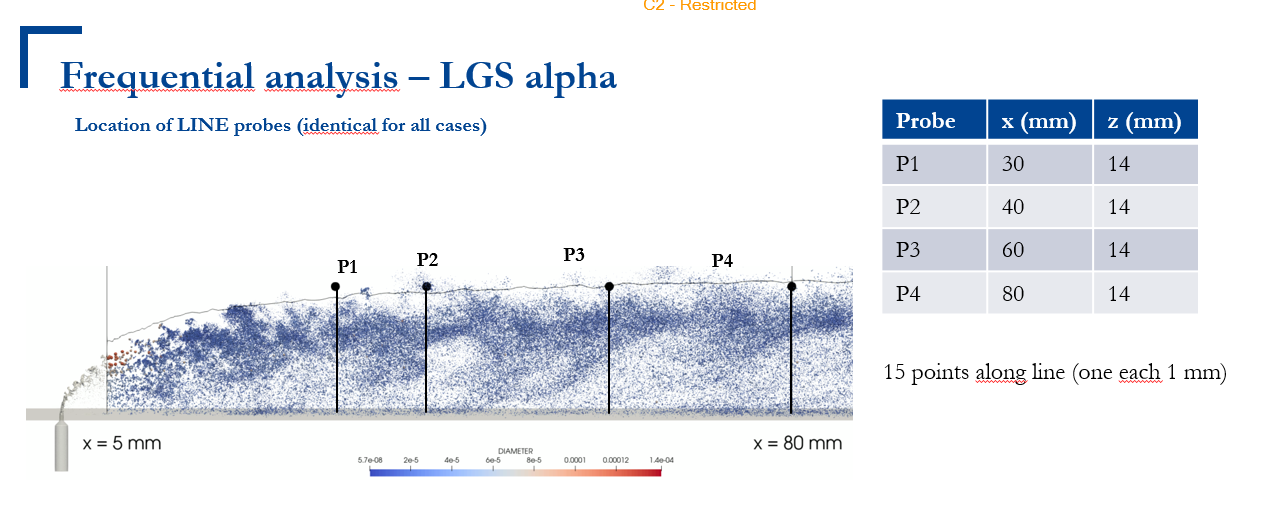
\includegraphics[scale=0.7]{./part2_developments/figures_ch6_lagrangian_JICF/probes_vol_frac}
	\caption{Probes for $\alpha$ frequential analysis for volume fraction}
	\label{fig:probes_dx10m}
\end{figure}


\begin{figure}[h!]
	\centering
	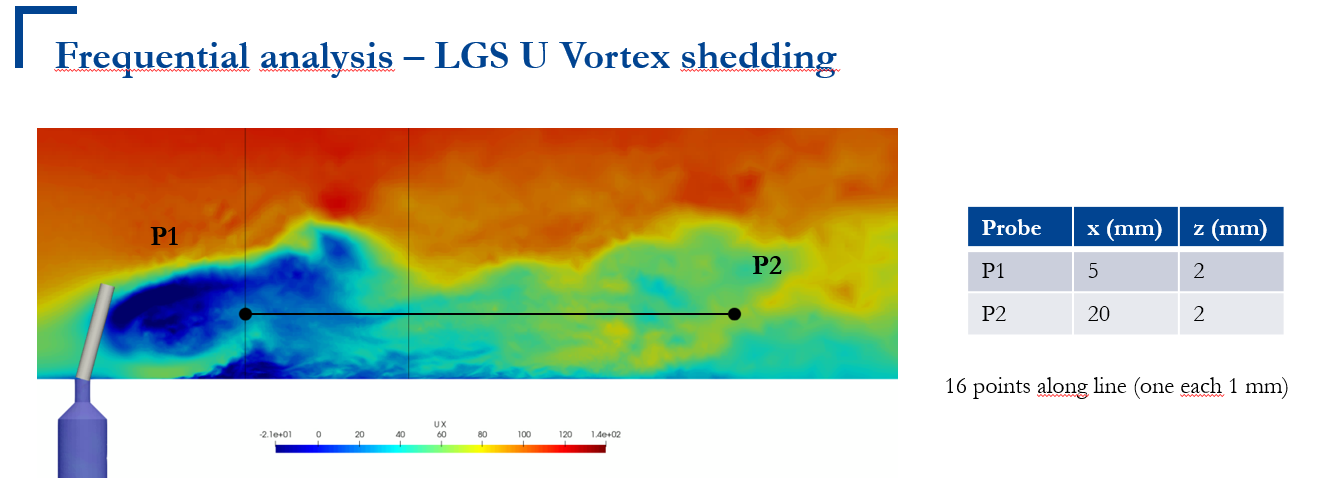
\includegraphics[scale=0.7]{./part2_developments/figures_ch6_lagrangian_JICF/probes_U_planey0}
	\caption{Probes for $U$ study}
	\label{fig:probes_U_planey0}
\end{figure}



\section{Conclusions}